\chapter{Graphrepräsentationen von Bildern}
\label{graphrepraesentationen_von_bildern}

Als eine \emph{Graphrepräsentation eines Bildes} $\gls{B} \in {\left[0, 1\right]}^{H \times W \times C}$ wird eine Darstellung von \gls{B} als ein gewichteter, ungerichteter sowie schleifenloser Graph \gls{G} verstanden, deren Knoten Informationen zu ausgewählten Bereichen von \gls{B} über eine Merkmalsmatrix $\ma{F} \in \gls{R}^{N \times M}$ speichern und deren Kanten eine Aussage über die örtlichen Nachbarschaften eines jeden Bildbereichs inne wohnt.
Formal lässt sich eine Graphrepräsentation eines Bildes damit als ein \emph{Graph im zweidimensionalen euklidischen Raum} $\gls{G} = \left(\gls{V}, \gls{E}, \gls{p}\right)$ verstehen, dem zusätzlich zu seinen Knoten- und Kantenmengen anstatt einer Gewichtsfunktion $\gls{w} \colon \gls{V} \times \gls{V} \to \gls{R}$ eine Positionsfunktion $\gls{p} \colon \gls{V} \to \gls{R}^2$ auf seinen Knoten in den zweidimensionalen euklidischen Raum $\gls{R}^2$ zugeordnet ist.
Das Gewicht $\gls{w} \colon \gls{E} \to \left[0, 1\right]$ einer Kante ergibt sich dann implizit als \enquote{Abstandsfunktion} mit Hilfe der euklidischen Norm $\left\|\cdot\right\|_2$ auf den Positionen des Knotens über
\begin{equation*}
  \left\|\gls{p}\left(\gls{v}_i\right) - \gls{p}\left(\gls{v}_j\right) \right\|_2 \coloneqq \sqrt{{\left({\gls{p}\left(\gls{v}_i\right)}_1 - {\gls{p}\left(\gls{v}_j\right)}_1\right)}^2 + {\left({\gls{p}\left(\gls{v}_i\right)}_2 - {\gls{p}\left(\gls{v}_j\right)}_2\right)}^2}
\end{equation*}
und der \emph{Gaußfunktion} als
\begin{equation}
  \gls{w}\left(\gls{v}_i, \gls{v}_j\right) \coloneqq \begin{cases}
    \exp\left(-\frac{\left\|\gls{p}\left(\gls{v}_i\right) - \gls{p}\left(\gls{v}_j\right)\right\|_2^2}{2\gls{sigma}^2}\right), & \text{wenn }\left(\gls{v}_i, \gls{v}_j\right) \in \gls{E},\\
    0, & \text{sonst},
  \end{cases}
  \label{gauss}
\end{equation}
wobei $\gls{sigma} \in \gls{R}$ ein frei wählbarer Parameter ist~\cite{Shuman}.
Abbildung~\ref{fig:gauss} veranschaulicht die Gewichtsfunktion anhand unterschiedlich gewählter $\gls{sigma}$.
\begin{figure}[t]
\centering
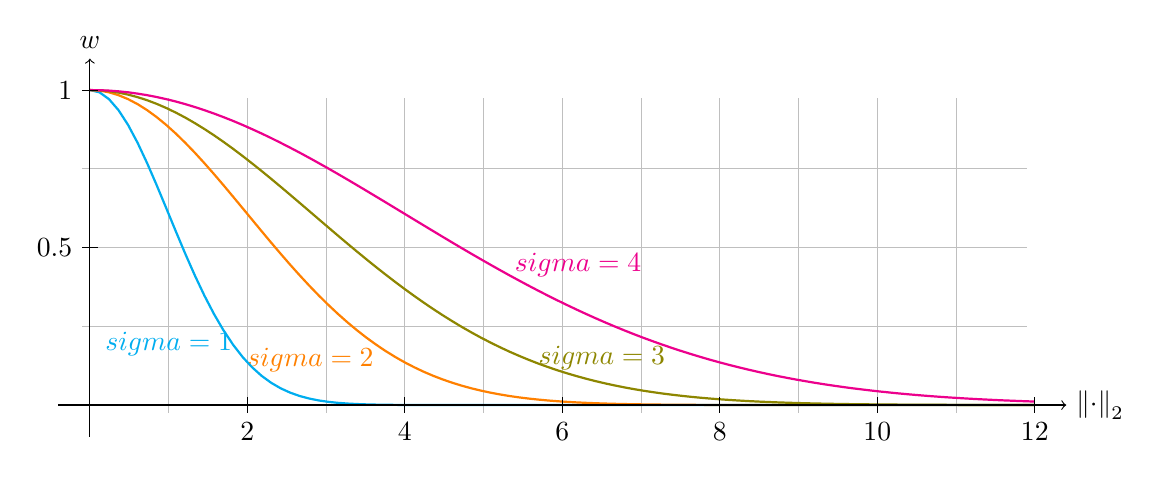
\begin{tikzpicture}
  \draw[color=lightgray] (-0.1, -0.1) grid (11.9, 3.9);
  \tikzstyle{color1}=[color=cyan]
  \tikzstyle{color2}=[color=orange]
  \tikzstyle{color3}=[color=olive]
  \tikzstyle{color4}=[color=magenta]

  \draw[color1] (1,0.5) node[above]   {$\gls{sigma} = 1$};
  \draw[color2] (2.8,0.3) node[above] {$\gls{sigma} = 2$};
  \draw[color3] (6.5,0.32) node[above] {$\gls{sigma} = 3$};
  \draw[color4] (6.2,1.5) node[above] {$\gls{sigma} = 4$};

  \draw [color1, thick,domain=0:12, samples=100] plot (\x,4*exp{-(\x)^2/2});  % 1
  \draw [color2, thick,domain=0:12, samples=100] plot (\x,4*exp{-(\x)^2/8});  % 2
  \draw [color3, thick,domain=0:12, samples=100] plot (\x,4*exp{-(\x)^2/16});  % 3
  \draw [color4, thick,domain=0:12, samples=100] plot (\x,4*exp{-(\x)^2/32});  % 4

  \draw[->] (-0.4, 0) -- (12.4, 0) node[right] {${\left\|\cdot\right\|}_2$};
  \draw[->] (0, -0.4) -- (0, 4.4) node[above] {$w$};
  \draw (0.1, 2) -- (-0.1, 2) node[left] {$0.5$};
  \draw (0.1, 4) -- (-0.1, 4) node[left] {$1$};
  \draw (2, 0.1) -- (2, -0.1) node[below] {$2$};
  \draw (4, 0.1) -- (4, -0.1) node[below] {$4$};
  \draw (6, 0.1) -- (6, -0.1) node[below] {$6$};
  \draw (8, 0.1) -- (8, -0.1) node[below] {$8$};
  \draw (10, 0.1) -- (10, -0.1) node[below] {$10$};
  \draw (12, 0.1) -- (12, -0.1) node[below] {$12$};

\end{tikzpicture}
  \caption[Kantengewichtsberechnung über Gaußfunktion]{Illustration der \enquote{invertierten} Kantengewichte $w \in \left[0, 1\right]$ basierend auf dessen Länge, gegeben durch die euklidische Norm ${\left\|\cdot\right\|}_2$.
  Je größer $\gls{sigma} \in \gls{R}$ gewählt, umso \enquote{stumpfer} zeichnet sich die Gaußfunktion und umso längere Kanten erhalten ein Gewicht $\gg 0$.
  Die Wahl von \gls{sigma} ist damit abhängig von der Ausdehnung der Distanzen eines Graphen.}
\label{fig:gauss}
\end{figure}

Aufgrund der Symmetrie von ${\left\|\cdot\right\|}_2$ folgt insbesondere sofort die Ungerichtheit des Graphen \gls{G}, \dhe{} $\gls{w}\left(\gls{v}_i, \gls{v}_j\right) = \gls{w}\left(\gls{v}_j, \gls{v}_i\right)$.
Die Gaußfunktion \enquote{invertiert} dabei den Abstand zweier Knoten zueinander, sodass Knoten die weiter voneinander entfernt liegen ein geringeres Gewicht besitzen.
Das korrespondiert mit dem üblichen Verständnis eines Kantengewichts in Graphen.
Knoten, die näher am Ursprungsknoten liegen, gelten als \enquote{wichtiger} und bekommen deshalb ein größeres Gewicht.
Insbesondere stimmt dies mit der Konvention überein, dass $\gls{w}\left(\gls{v}_i, \gls{v}_j\right) = 0$ für $\left(\gls{v}_i, \gls{v}_j\right) \notin \gls{E}$.
Damit lässt sich weiterhin die korrespondierende Adjazenzmatrix $\gls{Adist} \in \left[0, 1\right] \in \gls{R}^{N \times N}$ wie bekannt mit ${\left(\gls{Adist}\right)}_{ij} \coloneqq \gls{w}\left(\gls{v}_i, \gls{v}_j\right)$ definieren.

Zusätzlich zu dem Abstand der Knoten \bzw{} der Länge der Kanten eines Graphen im zweidimensionalen euklidischen Raum $\gls{G} = \left(\gls{V}, \gls{E}, \gls{p}\right)$ lassen sich die Ausrichtungen der Kanten über die Positionen der Knoten von \gls{G} festhalten.
Aus $p \colon \gls{V} \to \gls{R}$ wird folglich über
\begin{equation*}
  \gls{winkel}\left(\gls{v}_i, \gls{v}_j\right) \coloneqq \begin{cases}
    \mathrm{atan2}\left({\gls{p}\left(\gls{v}_j - \gls{v}_i\right)}_1, {\gls{p}\left(\gls{v}_j - \gls{v}_i\right)}_2\right) + \pi, & \text{wenn }\left(\gls{v}_i, \gls{v}_j\right) \in \gls{E},\\
    0, & \text{sonst}
  \end{cases}
\end{equation*}
eine \emph{Winkelfunktion} $\gls{winkel} \colon \gls{V} \times \gls{V} \to \left[0, 2\pi\right]$ auf den Kanten von \gls{G} im Uhrzeigersinn definiert, wobei $\mathrm{atan2}\left(x, y\right) \in \left[-\pi, \pi\right]$ den Arkustangens von $x/y$ berechnet, aber im Gegensatz zu $\mathrm{atan}\left(\cdot\right)$ die Vorzeichen beider Parameter beachtet und so den Quadranten des Ergebnisses bestimmen kann (\vgl{}~\cite{atan2}).
Der Winkel Null wird dabei explizit als $2\pi$ definiert, sodass weiterhin $\gls{winkel}\left(\gls{v}_i, \gls{v}_j\right) = 0$ gilt, falls $\left(\gls{v}_i, \gls{v}_j\right) \notin \gls{E}$.
Analog zu \gls{Adist} lässt sich damit die Adjazenzmatrix $\gls{Arad} \in {\left[0, 2\pi\right]}^{N \times N}$ mit ${\left(\gls{Arad}\right)}_{ij} \coloneqq \gls{winkel}\left(\gls{v}_i, \gls{v}_j\right)$ definieren.
Es ist anzumerken, dass die Winkelfunktion \gls{winkel} im Gegensatz zur Gewichtsfunktion \gls{w} nicht symmetrisch \bzw{} ungerichtet ist, \dhe{} $\gls{winkel}\left(\gls{v}_i, \gls{v}_i\right) \neq \gls{winkel}\left(\gls{v}_j, \gls{v}_i\right)$.
Insbesondere definiert \gls{Arad} damit einen gerichteten Graphen.

Die beiden Adjazenzmatrizen \gls{Adist} und \gls{Arad} beschreiben den Graphen $\gls{G} = \left(\gls{V}, \gls{E}, \gls{p}\right)$ bis auf Translation eindeutig.
Eine Veränderung einer Position $\gls{p}\left(\gls{v}\right)$ eines Knotens $\gls{v} \in \gls{V}$ führt sowohl zu einer Veränderung in \gls{Adist} als auch in \gls{Arad}.
Eine Translation aller Knoten um $\ve{\delta} \in \gls{R}^2$, \dhe{} $\gls{p}\left(\gls{v}\right) \rightarrow \gls{p}\left(\gls{v}\right) + \ve{\delta}$, generiert hingegen vollkommen äquivalente Adjazenzmatrizen \gls{Adist} sowie \gls{Arad}.
In der Regel ist dies kein Nachteil, denn nur in den seltensten Fällen interessieren uns die absoluten Positionen der Knoten in \gls{G}, wohingegen der Abstand und die Ausrichtungen der Knoten zueinander eine größere Bedeutung genießen.

Im Folgenden werden basierend auf der Definition eines Graphen im zweidimensionalen  euklidischen Raum zwei Ansätze für eine Graphrepräsentation von Bildern vorgestellt — der Repräsentation über ein reguläres Gitter sowie der Repräsentation über die Bestimmung von Superpixeln eines Bildes.

\section{Gitter}
\label{gitter}

Die einfachste Form einer Graphrepräsentation \gls{G} eines Bildes $\gls{B} \in \gls{R}^{H \times W \times C}$ ist die Repräsentation des Bildes über einen regulären Gittergraphen, denn dafür müssen keine Berechnungen am Bild vorgenommen werden.
Ein \emph{regulärer Gittergraph im zweidimensionalen euklidischen Raum} ist ein Graph $\gls{G} = \left(\gls{V}, \gls{E}, \gls{p}\right)$, der aus einem regulären Gitter gewonnen wurde und demnach genau $N \coloneqq H \times W$ Knoten enthält, \dhe{} einen Knoten für jedes Pixel in \gls{B}~\cite{Defferrard}.
Die Positionsfunktion der Knoten $\gls{p} \colon \gls{V} \to \gls{R}^2$ entspricht damit genau der Koordinate des korrespondierenden Pixels im Urpsprungsbild.
Sei dafür $\gls{v} \in \gls{V}$ der Knoten zu dem Bildpunkt an Position $\left(x,y\right)$.
Folglich gilt für die Position des Knotens $\gls{p}\left(\gls{v}\right) \coloneqq {\left[x,y\right]}^{\top}$.
Die örtlich um den Knoten $\gls{v} \in \gls{V}$ liegenden Knoten gelten dann auch im Gittergraph als benachbart und werden über eine Kante in \gls{E} verbunden.
Dabei unterscheidet man zwischen zwei frei wählbaren \emph{Konnektivitäten} des Graphen~\cite{Defferrard}.
Eine Konnektivität von $4$ bedeutet, dass ein Knoten (ohne Berücksichtigung der Randknoten) genau vier Nachbarn besitzt, die horizontal und vertikal zu im stehen.
Bei einer Konnektivität von $8$ gelten zusätzlich die vier diagonal zu ihm stehenden Knoten als Nachbarn und die Nachbarschaft wird folglich als ein $3 \times 3$ Fenster um den Knoten \gls{v} verstanden.

Analog zu den Daten der Farbkanäle an den einzelnen Pixeln des Bildes hängt auch an den Knoten über einer Merkmalsfunktion $f \colon \gls{V} \to \gls{R}^C$ \bzw{} einer Merkmalsmatrix $\ma{F} \in \gls{R}^{N \times C}$ diese Information mit $f\left(\gls{v}\right) \coloneqq \gls{B}_{{p\left(\gls{v}\right)}_2,{p\left(\gls{v}\right)}_1}$.

\paragraph{Effiziente Adjazenzbestimmung}
\label{adjazenzbestimmung_gitter}

Entgegen der Pixelanordnung in einem Bild ist die Anordnung der Knoten in einem Gittergraphen völlig irrelevant und kann willkürlich gewählt werden.
Ein Aufbau der Kantenmenge \gls{E} \bzw{} der korrespondierenden, ungewichteten Adjazenzmatrix \gls{A} kann jedoch besonders effizient gestaltet werden, wenn die Knoten reihenweise entsprechend ihrer Bildkoordinate angeordnet werden.
Dafür wird das Bild \gls{B} zunächst an dessen Rändern um eine zusätzliche Spalte \bzw{} Reihe erweitert, \dhe{} $\gls{B} \in {\left[0, 1\right]}^{\left(H + 2\right) \times \left(W + 2\right) \times C}$.
Dann besitzt die ungewichtete Adjazenzmatrix $\gls{A} \in {\left\{0, 1\right\}}^{N \times N}$ mit $N \coloneqq \left(H+2\right)\left(W+2\right)$ in den Reihen $W+3 < i < N - W - 3$ an den Spaltenindizes $\left\{i-W-2, i-1, i+1, i+W+2\right\}$ \bzw{}
\begin{equation*}
  \left\{i-W-3, i-W-2, i-W-1, i-1, i+1, i+W+1, i+W+2, i+W+3\right\}
\end{equation*}
genau einen Eintrag gleich Eins (bei einer Konnektivität von $4$ \bzw{} $8$).
Anschließend müssen die ungültigen Knoten aus \gls{A} reihen- und spaltenweise schrittweise über eine Länge von $W$ mit Schrittweite $W+2$ gefiltert werden.
Dabei müssen natürlich zunächst die ersten und letzten $W + 3$ Knoten aus \gls{A} gelöscht werden.

\begin{figure}[t]
\centering
\subfigure[\gls{SLIC}]{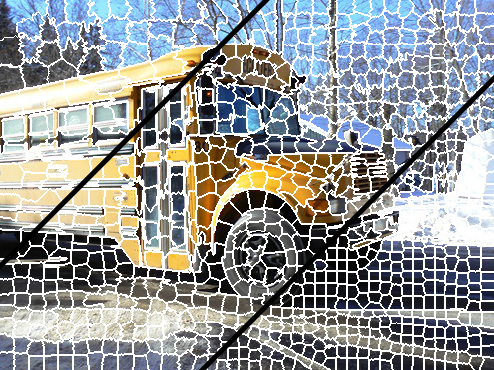
\includegraphics[scale=0.4]{bilder/slic_beispiel}}
\subfigure[Quickshift]{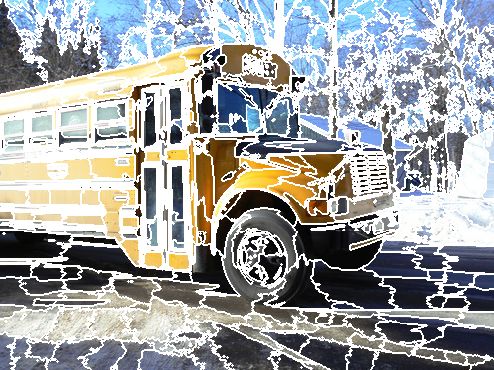
\includegraphics[scale=0.4]{bilder/quickshift_beispiel}}
  \caption[\gls{SLIC} und Quickshift Beispielresultat]{Ein Bus segmentiert über \gls{SLIC} mit jeweils 400, 800 und 1600 Superpixeln (a) sowie über Quickshift mit 600 Superpixeln (b).
  Dabei werden die unterschiedlichen Verfahren zur Generierung von Superpixeln deutlich.
  Wohingegen \gls{SLIC} möglichst quadratische, gleichgroße Superpixel erzeugt, wird die Form der Superpixel von Quickshift größtenteils über die Farbabgrenzungen gesteuert und erzeugt damit sowohl sehr große wie auch sehr kleine Superpixel in allen möglichen Variationen.}
\label{fig:slic_quickshift}
\end{figure}

